\documentclass[]{article}
\usepackage{lmodern}
\usepackage{amssymb,amsmath}
\usepackage{ifxetex,ifluatex}
\usepackage{fixltx2e} % provides \textsubscript
\ifnum 0\ifxetex 1\fi\ifluatex 1\fi=0 % if pdftex
  \usepackage[T1]{fontenc}
  \usepackage[utf8]{inputenc}
\else % if luatex or xelatex
  \ifxetex
    \usepackage{mathspec}
  \else
    \usepackage{fontspec}
  \fi
  \defaultfontfeatures{Ligatures=TeX,Scale=MatchLowercase}
\fi
% use upquote if available, for straight quotes in verbatim environments
\IfFileExists{upquote.sty}{\usepackage{upquote}}{}
% use microtype if available
\IfFileExists{microtype.sty}{%
\usepackage{microtype}
\UseMicrotypeSet[protrusion]{basicmath} % disable protrusion for tt fonts
}{}
\usepackage[margin=1in]{geometry}
\usepackage{hyperref}
\hypersetup{unicode=true,
            pdftitle={MATH1318 Time Series},
            pdfauthor={Phil Steinke s3725547},
            pdfborder={0 0 0},
            breaklinks=true}
\urlstyle{same}  % don't use monospace font for urls
\usepackage{color}
\usepackage{fancyvrb}
\newcommand{\VerbBar}{|}
\newcommand{\VERB}{\Verb[commandchars=\\\{\}]}
\DefineVerbatimEnvironment{Highlighting}{Verbatim}{commandchars=\\\{\}}
% Add ',fontsize=\small' for more characters per line
\usepackage{framed}
\definecolor{shadecolor}{RGB}{248,248,248}
\newenvironment{Shaded}{\begin{snugshade}}{\end{snugshade}}
\newcommand{\AlertTok}[1]{\textcolor[rgb]{0.94,0.16,0.16}{#1}}
\newcommand{\AnnotationTok}[1]{\textcolor[rgb]{0.56,0.35,0.01}{\textbf{\textit{#1}}}}
\newcommand{\AttributeTok}[1]{\textcolor[rgb]{0.77,0.63,0.00}{#1}}
\newcommand{\BaseNTok}[1]{\textcolor[rgb]{0.00,0.00,0.81}{#1}}
\newcommand{\BuiltInTok}[1]{#1}
\newcommand{\CharTok}[1]{\textcolor[rgb]{0.31,0.60,0.02}{#1}}
\newcommand{\CommentTok}[1]{\textcolor[rgb]{0.56,0.35,0.01}{\textit{#1}}}
\newcommand{\CommentVarTok}[1]{\textcolor[rgb]{0.56,0.35,0.01}{\textbf{\textit{#1}}}}
\newcommand{\ConstantTok}[1]{\textcolor[rgb]{0.00,0.00,0.00}{#1}}
\newcommand{\ControlFlowTok}[1]{\textcolor[rgb]{0.13,0.29,0.53}{\textbf{#1}}}
\newcommand{\DataTypeTok}[1]{\textcolor[rgb]{0.13,0.29,0.53}{#1}}
\newcommand{\DecValTok}[1]{\textcolor[rgb]{0.00,0.00,0.81}{#1}}
\newcommand{\DocumentationTok}[1]{\textcolor[rgb]{0.56,0.35,0.01}{\textbf{\textit{#1}}}}
\newcommand{\ErrorTok}[1]{\textcolor[rgb]{0.64,0.00,0.00}{\textbf{#1}}}
\newcommand{\ExtensionTok}[1]{#1}
\newcommand{\FloatTok}[1]{\textcolor[rgb]{0.00,0.00,0.81}{#1}}
\newcommand{\FunctionTok}[1]{\textcolor[rgb]{0.00,0.00,0.00}{#1}}
\newcommand{\ImportTok}[1]{#1}
\newcommand{\InformationTok}[1]{\textcolor[rgb]{0.56,0.35,0.01}{\textbf{\textit{#1}}}}
\newcommand{\KeywordTok}[1]{\textcolor[rgb]{0.13,0.29,0.53}{\textbf{#1}}}
\newcommand{\NormalTok}[1]{#1}
\newcommand{\OperatorTok}[1]{\textcolor[rgb]{0.81,0.36,0.00}{\textbf{#1}}}
\newcommand{\OtherTok}[1]{\textcolor[rgb]{0.56,0.35,0.01}{#1}}
\newcommand{\PreprocessorTok}[1]{\textcolor[rgb]{0.56,0.35,0.01}{\textit{#1}}}
\newcommand{\RegionMarkerTok}[1]{#1}
\newcommand{\SpecialCharTok}[1]{\textcolor[rgb]{0.00,0.00,0.00}{#1}}
\newcommand{\SpecialStringTok}[1]{\textcolor[rgb]{0.31,0.60,0.02}{#1}}
\newcommand{\StringTok}[1]{\textcolor[rgb]{0.31,0.60,0.02}{#1}}
\newcommand{\VariableTok}[1]{\textcolor[rgb]{0.00,0.00,0.00}{#1}}
\newcommand{\VerbatimStringTok}[1]{\textcolor[rgb]{0.31,0.60,0.02}{#1}}
\newcommand{\WarningTok}[1]{\textcolor[rgb]{0.56,0.35,0.01}{\textbf{\textit{#1}}}}
\usepackage{graphicx,grffile}
\makeatletter
\def\maxwidth{\ifdim\Gin@nat@width>\linewidth\linewidth\else\Gin@nat@width\fi}
\def\maxheight{\ifdim\Gin@nat@height>\textheight\textheight\else\Gin@nat@height\fi}
\makeatother
% Scale images if necessary, so that they will not overflow the page
% margins by default, and it is still possible to overwrite the defaults
% using explicit options in \includegraphics[width, height, ...]{}
\setkeys{Gin}{width=\maxwidth,height=\maxheight,keepaspectratio}
\IfFileExists{parskip.sty}{%
\usepackage{parskip}
}{% else
\setlength{\parindent}{0pt}
\setlength{\parskip}{6pt plus 2pt minus 1pt}
}
\setlength{\emergencystretch}{3em}  % prevent overfull lines
\providecommand{\tightlist}{%
  \setlength{\itemsep}{0pt}\setlength{\parskip}{0pt}}
\setcounter{secnumdepth}{0}
% Redefines (sub)paragraphs to behave more like sections
\ifx\paragraph\undefined\else
\let\oldparagraph\paragraph
\renewcommand{\paragraph}[1]{\oldparagraph{#1}\mbox{}}
\fi
\ifx\subparagraph\undefined\else
\let\oldsubparagraph\subparagraph
\renewcommand{\subparagraph}[1]{\oldsubparagraph{#1}\mbox{}}
\fi

%%% Use protect on footnotes to avoid problems with footnotes in titles
\let\rmarkdownfootnote\footnote%
\def\footnote{\protect\rmarkdownfootnote}

%%% Change title format to be more compact
\usepackage{titling}

% Create subtitle command for use in maketitle
\newcommand{\subtitle}[1]{
  \posttitle{
    \begin{center}\large#1\end{center}
    }
}

\setlength{\droptitle}{-2em}

  \title{MATH1318 Time Series}
    \pretitle{\vspace{\droptitle}\centering\huge}
  \posttitle{\par}
  \subtitle{Assignment 2 - Semester 1, 2019}
  \author{Phil Steinke s3725547}
    \preauthor{\centering\large\emph}
  \postauthor{\par}
    \date{}
    \predate{}\postdate{}
  

\begin{document}
\maketitle

\hypertarget{executive-summary}{%
\subsection{Executive Summary}\label{executive-summary}}

\hypertarget{reporting-15}\label{reporting-15}}

\hypertarget{data}{%
\subsubsection{Data}\label{data}}

Egg depositions (in millions) of age-3
\href{https://en.wikipedia.org/wiki/Coregonus_hoyi}{Lake Huron Bloaters
(Coregonus hoyi)} between years 1981 and 1996 are available in BloaterLH
dataset of FSAdata package.

\hypertarget{goals}{%
\subsubsection{Goals}\label{goals}}

\begin{itemize}
\tightlist
\item[$\boxtimes$]
  Analyse the egg depositions of Lake Huron Bloasters
\item[$\boxtimes$]
  Use the analysis methods covered in the \textbf{modules 1 -- 7} of
  MATH1318 Time Series Analysis
\item[$\square$]
  Choose the best model among a set of possible models for this dataset
\item
  {[}-{]} Give forecasts of egg depositions for the next 5 years
\end{itemize}

\hypertarget{r-code-15}\label{r-code-15}}

\begin{Shaded}
\begin{Highlighting}[]
\KeywordTok{cat}\NormalTok{(}\StringTok{"}\CharTok{\textbackslash{}014}\StringTok{"}\NormalTok{) }\CommentTok{# clear everything}
\end{Highlighting}
\end{Shaded}



\begin{Shaded}
\begin{Highlighting}[]
\KeywordTok{setwd}\NormalTok{(}\StringTok{"./."}\NormalTok{)}
\NormalTok{dataFilename <-}\StringTok{ "raw-data/eggs.csv"}
\NormalTok{startYear =}\StringTok{ }\DecValTok{1981} \CommentTok{# get start year}
\NormalTok{endYear =}\StringTok{ }\DecValTok{1996} \CommentTok{# get end year}
\CommentTok{# install with `devtools::install_git('https://gitlab.com/botbotdotdotcom/packagr')`}
\KeywordTok{library}\NormalTok{(packagr)}
\NormalTok{packages <-}\StringTok{ }\KeywordTok{c}\NormalTok{(}\StringTok{'FitAR'}\NormalTok{,}\StringTok{'fUnitRoots'}\NormalTok{,}\StringTok{'lmtest'}\NormalTok{,}\StringTok{'readr'}\NormalTok{,}\StringTok{'tidyr'}\NormalTok{,}\StringTok{'TSA'}\NormalTok{,}\StringTok{'TTR'}\NormalTok{,}\StringTok{'MASS'}\NormalTok{,}\StringTok{'purrr'}\NormalTok{, }\StringTok{'captioner'}\NormalTok{)}
\KeywordTok{packagr}\NormalTok{(packages) }\CommentTok{# alpha package to check, install and load packages}
\NormalTok{data <-}\StringTok{ }\KeywordTok{read_csv}\NormalTok{(dataFilename)}
\CommentTok{# convert to timeseries, ignoring year column:}
\NormalTok{data.ts <-}\StringTok{ }\KeywordTok{ts}\NormalTok{(}\KeywordTok{as.vector}\NormalTok{(data[,}\DecValTok{2}\NormalTok{]), }\DataTypeTok{start =}\NormalTok{ startYear, }\DataTypeTok{end =}\NormalTok{ endYear) }
\KeywordTok{source}\NormalTok{(}\StringTok{'~/code/data-science/uni/time-series/common/sort.score.R'}\NormalTok{)}
\NormalTok{data.ts.raw <-}\StringTok{ }\NormalTok{data.ts }\CommentTok{# make a copy for forecasting}
\end{Highlighting}
\end{Shaded}

\begin{Shaded}
\begin{Highlighting}[]
\CommentTok{# class(data) -> ts}
\CommentTok{# data %>% dim() # 16 x 2 }
\NormalTok{data.ts }\OperatorTok\StringTok{ }\KeywordTok{dim}\NormalTok{() }\CommentTok{# 16 x 1 because we removed the year column}
\end{Highlighting}
\end{Shaded}

\begin{verbatim}
## [1] 16  1
\end{verbatim}

\begin{Shaded}
\begin{Highlighting}[]
\NormalTok{default_ylab =}\StringTok{ 'Lake Huron Bloaters'}
\NormalTok{default_xlab =}\StringTok{ 'Year'}
\NormalTok{fig_nums <-}\StringTok{ }\KeywordTok{captioner}\NormalTok{()}

\NormalTok{doDiffAndPlot <-}\StringTok{ }\ControlFlowTok{function}\NormalTok{(df.ts, diffCount, }\DataTypeTok{showPlot =}\NormalTok{ T, }\DataTypeTok{showEacf=}\NormalTok{F) \{}
  \KeywordTok{ifelse}\NormalTok{(}
\NormalTok{    diffCount }\OperatorTok{!=}\StringTok{ }\DecValTok{0}\NormalTok{, (}\DataTypeTok{df.ts =} \KeywordTok{diff}\NormalTok{(df.ts, }\DataTypeTok{differences =}\NormalTok{ diffCount)),}
    \StringTok{'there is no diff}\CharTok{\textbackslash{}n}\StringTok{'}\NormalTok{)}
  \KeywordTok{paste}\NormalTok{(}\StringTok{'diff: '}\NormalTok{, diffCount) }\OperatorTok\StringTok{ }\KeywordTok{print}\NormalTok{()}
\NormalTok{  order =}\StringTok{ }\KeywordTok{ar}\NormalTok{(}\KeywordTok{diff}\NormalTok{(df.ts))}\OperatorTok{$}\NormalTok{order}
  \KeywordTok{paste}\NormalTok{(}\StringTok{'order count (k): '}\NormalTok{, order)}
\NormalTok{  diffAdfTest =}\StringTok{ }\KeywordTok{adfTest}\NormalTok{(df.ts, }\DataTypeTok{lags =}\NormalTok{ order, }\DataTypeTok{title =} \OtherTok{NULL}\NormalTok{, }\DataTypeTok{description =} \OtherTok{NULL}\NormalTok{)}
\NormalTok{  p <-}\StringTok{ }\NormalTok{diffAdfTest}\OperatorTok{@}\NormalTok{test}\OperatorTok{$}\NormalTok{p.value}
  \KeywordTok{paste}\NormalTok{(}
    \StringTok{'adf p-value:'}\NormalTok{,}
\NormalTok{    p, (}\KeywordTok{ifelse}\NormalTok{(p }\OperatorTok{<}\StringTok{ }\FloatTok{0.05}\NormalTok{, }\StringTok{'< 0.05 significant'}\NormalTok{, }\StringTok{'> 0.05 insignificant'}\NormalTok{)}
\NormalTok{    )) }\OperatorTok\StringTok{ }\KeywordTok{print}\NormalTok{()}
  \CommentTok{# }\AlertTok{~old_todo~}\CommentTok{: later ifelse(showEacf, eacf(df.ts, ar.max=3, ma.max=3),'') # works on larger datasets}
  \ControlFlowTok{if}\NormalTok{(showPlot) \{}
    \KeywordTok{par}\NormalTok{(}\DataTypeTok{mfrow =} \KeywordTok{c}\NormalTok{(}\DecValTok{1}\NormalTok{,}\DecValTok{3}\NormalTok{))}
    \KeywordTok{plot}\NormalTok{(}
\NormalTok{      df.ts, }
      \DataTypeTok{type=}\StringTok{'o'}\NormalTok{, }
      \DataTypeTok{xlab=}\NormalTok{default_xlab, }
      \CommentTok{# ylab=fig_nums(figureName, }
      \CommentTok{#   paste('diff #', diffCount, ' of ', default_ylab, sep = '')}
      \CommentTok{# )}
\NormalTok{    )}
    \KeywordTok{acf}\NormalTok{(df.ts)}
    \KeywordTok{pacf}\NormalTok{(df.ts)}
    \KeywordTok{par}\NormalTok{(}\DataTypeTok{mfrow=}\KeywordTok{c}\NormalTok{(}\DecValTok{1}\NormalTok{,}\DecValTok{1}\NormalTok{))}
\NormalTok{  \}}

\NormalTok{\}}
\end{Highlighting}
\end{Shaded}

\begin{Shaded}
\begin{Highlighting}[]
\CommentTok{# The initial ts data, without any transformation:}
\KeywordTok{fig_nums}\NormalTok{(}\StringTok{'initial ts data'}\NormalTok{, }\StringTok{'initial timeseries data with no transformation'}\NormalTok{) }\OperatorTok\StringTok{ }\KeywordTok{cat}\NormalTok{()}
\end{Highlighting}
\end{Shaded}

\begin{verbatim}
## Figure  1: initial timeseries data with no transformation
\end{verbatim}

\begin{Shaded}
\begin{Highlighting}[]
\KeywordTok{doDiffAndPlot}\NormalTok{(data.ts, }\DecValTok{0}\NormalTok{, T, F) }\CommentTok{# p = 0.4455 lag = 1 - has a trend = nope}
\end{Highlighting}
\end{Shaded}

\begin{verbatim}
## [1] "diff:  0"
## [1] "adf p-value: 0.452033577643409 > 0.05 insignificant"
\end{verbatim}

\includegraphics{assignment02-psteinke-timeseries_files/figure-latex/initial-data-1.pdf}

\begin{itemize}
\tightlist
\item
  Plot has visual positive trend
\item
  Small dataset, so it is hard to visually observe any significant
  seasonality
\item
  ACF and PACF have a waveform (similar to sin/cosine wave)
\item
  Has a clear lag of 1 in ACF and PACF
\end{itemize}

\hypertarget{confidence-interval}{%
\subsection{Confidence interval}\label{confidence-interval}}

\begin{Shaded}
\begin{Highlighting}[]
\CommentTok{# check the confidence interval of BoxCox}
\KeywordTok{fig_nums}\NormalTok{(}\StringTok{"confidence-interval"}\NormalTok{, }\KeywordTok{paste}\NormalTok{(}\StringTok{'Confidence Interval for '}\NormalTok{, default_ylab, }\DataTypeTok{sep =} \StringTok{''}\NormalTok{)) }\OperatorTok\StringTok{ }\KeywordTok{cat}\NormalTok{()}
\end{Highlighting}
\end{Shaded}

\begin{verbatim}
## Figure  2: Confidence Interval for Lake Huron Bloaters
\end{verbatim}

\begin{Shaded}
\begin{Highlighting}[]
\NormalTok{boxcoxCi <-}\StringTok{ }\KeywordTok{BoxCox.ar}\NormalTok{(data.ts, }\DataTypeTok{method =} \StringTok{"yule-walker"}\NormalTok{)}\OperatorTok{$}\NormalTok{ci}
\end{Highlighting}
\end{Shaded}

\includegraphics{assignment02-psteinke-timeseries_files/figure-latex/confidence-interval-1.pdf}

\begin{itemize}
\tightlist
\item
  The confidence interval \texttt{0.1\ -\ 0.8} does not include 0, so we
  \emph{cannot} do a log transform
\end{itemize}

\begin{Shaded}
\begin{Highlighting}[]
\NormalTok{doTestNormality <-}\StringTok{ }\ControlFlowTok{function}\NormalTok{(df) \{}
  \KeywordTok{qqnorm}\NormalTok{(df)}
  \KeywordTok{qqline}\NormalTok{(df, }\DataTypeTok{col =} \DecValTok{2}\NormalTok{)}
  \KeywordTok{shapiro.test}\NormalTok{(df)}
\NormalTok{\}}
\NormalTok{lambda <-}\StringTok{ }\NormalTok{(}\KeywordTok{max}\NormalTok{(boxcoxCi)}\OperatorTok{-}\KeywordTok{min}\NormalTok{(boxcoxCi))}\OperatorTok{/}\DecValTok{2} 
\CommentTok{# lambda=0.35 ~midpoint betwen confidence interval (0.8-0.1)/2}
\NormalTok{data.ts.boxcox =}\StringTok{ }\NormalTok{(data.ts}\OperatorTok{^}\NormalTok{lambda}\DecValTok{-1}\NormalTok{) }\OperatorTok{/}\StringTok{ }\NormalTok{lambda }
\KeywordTok{fig_nums}\NormalTok{(}\StringTok{"test-normality"}\NormalTok{, }\KeywordTok{paste}\NormalTok{(}\StringTok{'Test Normality of '}\NormalTok{, default_ylab, }\DataTypeTok{sep =} \StringTok{''}\NormalTok{)) }\OperatorTok\StringTok{ }\KeywordTok{cat}\NormalTok{()}
\end{Highlighting}
\end{Shaded}

\begin{verbatim}
## Figure  3: Test Normality of Lake Huron Bloaters
\end{verbatim}

\begin{Shaded}
\begin{Highlighting}[]
\KeywordTok{doTestNormality}\NormalTok{(data.ts.boxcox)}
\end{Highlighting}
\end{Shaded}

\includegraphics{assignment02-psteinke-timeseries_files/figure-latex/test-normality-1.pdf}

\begin{verbatim}
## 
##  Shapiro-Wilk normality test
## 
## data:  df
## W = 0.95345, p-value = 0.5463
\end{verbatim}

The Box-Cox transformation \textbf{did} help to improve the normality of
the series because: - the dots are moreso aligned with the red line in
the QQ plot - However, it isn't a perfect fit with QQ between
\textasciitilde(-2:0.5) does not fitting the QQ plot line - The Shapiro
test p-value(0.5463) \textgreater{} 0.05 - Possible intonation point or
bimodal data in the data

\hypertarget{diff}{%
\subsection{Diff}\label{diff}}

\hypertarget{without-box-cox}{%
\subsubsection{Without Box-Cox}\label{without-box-cox}}

\begin{Shaded}
\begin{Highlighting}[]
\KeywordTok{doDiffAndPlot}\NormalTok{(data.ts, }\DecValTok{1}\NormalTok{, F, F) }\CommentTok{# p = 0.3601 no lags! = nope }\AlertTok{~old_todo~}\CommentTok{: only show lags}
\end{Highlighting}
\end{Shaded}

\begin{verbatim}
## [1] "diff:  1"
## [1] "adf p-value: 0.360073649761517 > 0.05 insignificant"
\end{verbatim}

\begin{Shaded}
\begin{Highlighting}[]
\KeywordTok{doDiffAndPlot}\NormalTok{(data.ts, }\DecValTok{2}\NormalTok{, F) }\CommentTok{# p = 0.1643 lag = 4 = p is insignificant}
\end{Highlighting}
\end{Shaded}

\begin{verbatim}
## [1] "diff:  2"
## [1] "adf p-value: 0.164314242031066 > 0.05 insignificant"
\end{verbatim}

\begin{Shaded}
\begin{Highlighting}[]
\KeywordTok{doDiffAndPlot}\NormalTok{(data.ts, }\DecValTok{3}\NormalTok{, F, F) }\CommentTok{# p = 0.3768 lag = 1, 4 = p is significant}
\end{Highlighting}
\end{Shaded}

\begin{verbatim}
## [1] "diff:  3"
## [1] "adf p-value: 0.376694692418674 > 0.05 insignificant"
\end{verbatim}

\begin{itemize}
\tightlist
\item
  Our third diff doesn't add any further value
\item
  Best is second diff with p 0.1643
\item
  EACF We can't see any meaningful shelf, which indicates white noise
  series and possible non-stationarity
\end{itemize}

\hypertarget{diff-1}{%
\subsection{Diff}\label{diff-1}}

\hypertarget{with-box-cox}{%
\subsubsection{With Box-Cox}\label{with-box-cox}}

\begin{Shaded}
\begin{Highlighting}[]
\KeywordTok{fig_nums}\NormalTok{(}\StringTok{'boxCox diff 0'}\NormalTok{, }\StringTok{'BoxCox without any diff'}\NormalTok{) }\OperatorTok\StringTok{ }\KeywordTok{cat}\NormalTok{()}
\end{Highlighting}
\end{Shaded}

\begin{verbatim}
## Figure  4: BoxCox without any diff
\end{verbatim}

\begin{Shaded}
\begin{Highlighting}[]
\KeywordTok{doDiffAndPlot}\NormalTok{(data.ts.boxcox, }\DecValTok{0}\NormalTok{, T) }\CommentTok{# p < 0.05 = 0.01941, lag = 1 but it still has trend}
\end{Highlighting}
\end{Shaded}

\begin{verbatim}
## [1] "diff:  0"
## [1] "adf p-value: 0.0224250337343733 < 0.05 significant"
\end{verbatim}

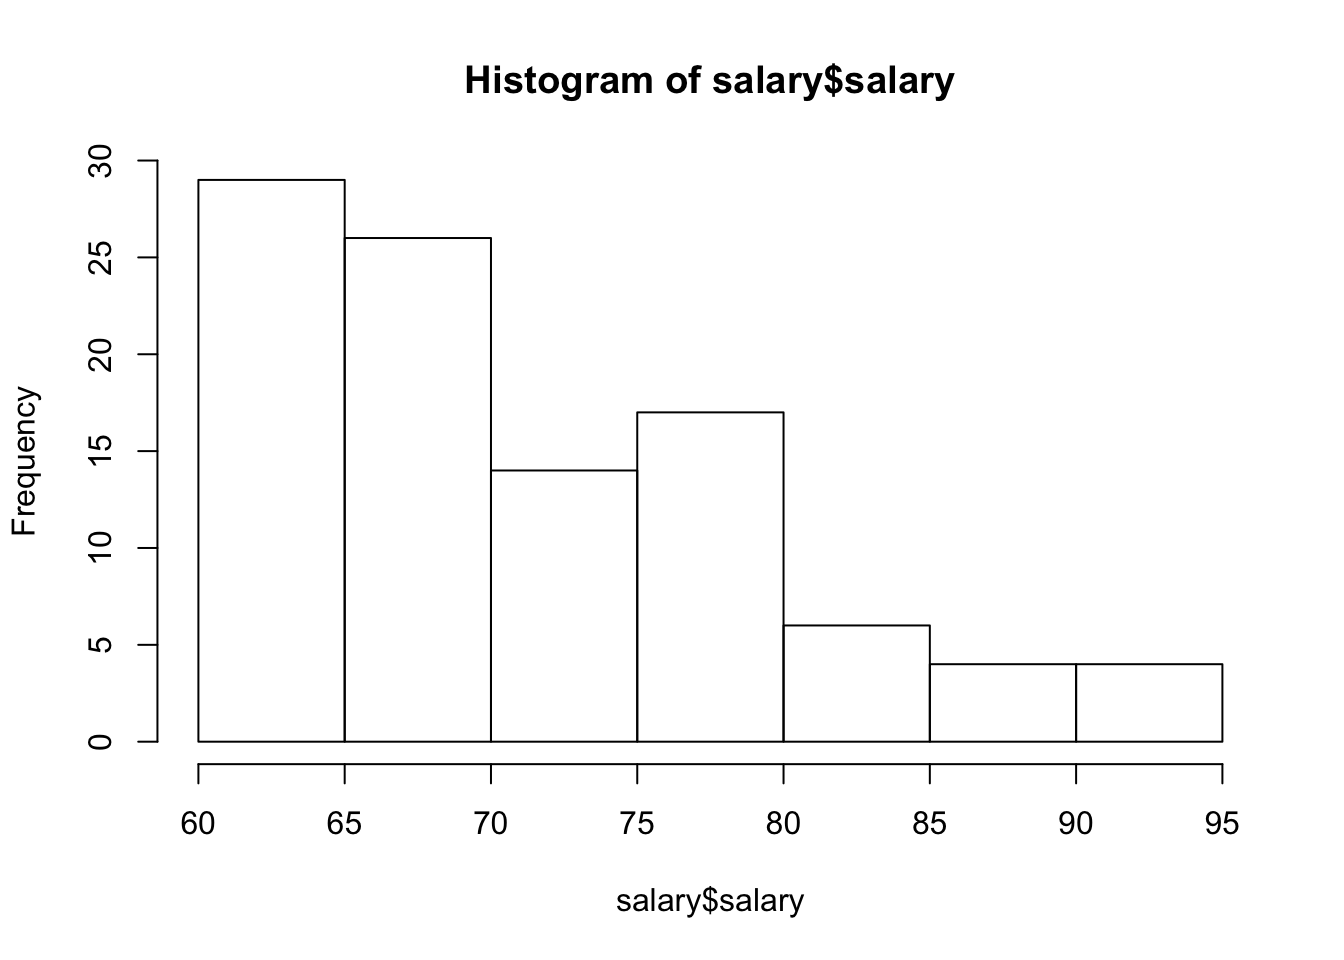
\includegraphics{assignment02-psteinke-timeseries_files/figure-latex/unnamed-chunk-1-1.pdf}

\begin{Shaded}
\begin{Highlighting}[]
\KeywordTok{doDiffAndPlot}\NormalTok{(data.ts.boxcox, }\DecValTok{1}\NormalTok{, F) }\CommentTok{# p is higher 0.3282, better trend! Looks stationary}
\end{Highlighting}
\end{Shaded}

\begin{verbatim}
## [1] "diff:  1"
## [1] "adf p-value: 0.328249580787965 > 0.05 insignificant"
\end{verbatim}

\begin{Shaded}
\begin{Highlighting}[]
\KeywordTok{doDiffAndPlot}\NormalTok{(data.ts.boxcox, }\DecValTok{2}\NormalTok{, F) }\CommentTok{# p is better 0.09166 pacf lag of 1 @4 pacf}
\end{Highlighting}
\end{Shaded}

\begin{verbatim}
## [1] "diff:  2"
## [1] "adf p-value: 0.0916630459959721 > 0.05 insignificant"
\end{verbatim}

\begin{Shaded}
\begin{Highlighting}[]
\KeywordTok{doDiffAndPlot}\NormalTok{(data.ts.boxcox, }\DecValTok{3}\NormalTok{, F) }\CommentTok{# p is better 0.14 pacf lag of 1 @4 pacf}
\end{Highlighting}
\end{Shaded}

\begin{verbatim}
## [1] "diff:  3"
## [1] "adf p-value: 0.141211776292504 > 0.05 insignificant"
\end{verbatim}

\begin{Shaded}
\begin{Highlighting}[]
\KeywordTok{fig_nums}\NormalTok{(}\StringTok{'boxCox diff 4'}\NormalTok{, }\StringTok{'BoxCox with diff of 4'}\NormalTok{) }\OperatorTok\StringTok{ }\KeywordTok{cat}\NormalTok{()}
\end{Highlighting}
\end{Shaded}

\begin{verbatim}
## Figure  5: BoxCox with diff of 4
\end{verbatim}

\begin{Shaded}
\begin{Highlighting}[]
\KeywordTok{doDiffAndPlot}\NormalTok{(data.ts.boxcox, }\DecValTok{4}\NormalTok{, T, F) }\CommentTok{# p is better 0.02 pacf lag of 1 @4 pacf}
\end{Highlighting}
\end{Shaded}

\begin{verbatim}
## [1] "diff:  4"
## [1] "adf p-value: 0.0199702709567182 < 0.05 significant"
\end{verbatim}

\includegraphics{assignment02-psteinke-timeseries_files/figure-latex/unnamed-chunk-1-2.pdf}

\begin{itemize}
\tightlist
\item
  Box-Cox transform has significance
  \texttt{p-value\ \textless{}\ 0.05\ =\ 0.01941}
\item
  Box-Cox transform with 4 differences has significance
  \texttt{p-value\ \textless{}\ 0.05\ =\ 0.01997}
\item
  Box-Cox with no difference still shows a trend ∴ we select Box-Cox
  with a diff(4):
\end{itemize}

\begin{Shaded}
\begin{Highlighting}[]
\CommentTok{# set variable for model testing:}
\NormalTok{data.ts.boxcox4 <-}\KeywordTok{diff}\NormalTok{(data.ts.boxcox, }\DataTypeTok{difference =} \DecValTok{4}\NormalTok{)}
\KeywordTok{fig_nums}\NormalTok{(}\StringTok{'Normal Q-Q Plot test'}\NormalTok{, }\StringTok{'Normal Q-Q Plot test'}\NormalTok{) }\OperatorTok\StringTok{ }\KeywordTok{cat}\NormalTok{()}
\end{Highlighting}
\end{Shaded}

\begin{verbatim}
## Figure  6: Normal Q-Q Plot test
\end{verbatim}

\begin{Shaded}
\begin{Highlighting}[]
\KeywordTok{doTestNormality}\NormalTok{(data.ts.boxcox4)}
\end{Highlighting}
\end{Shaded}

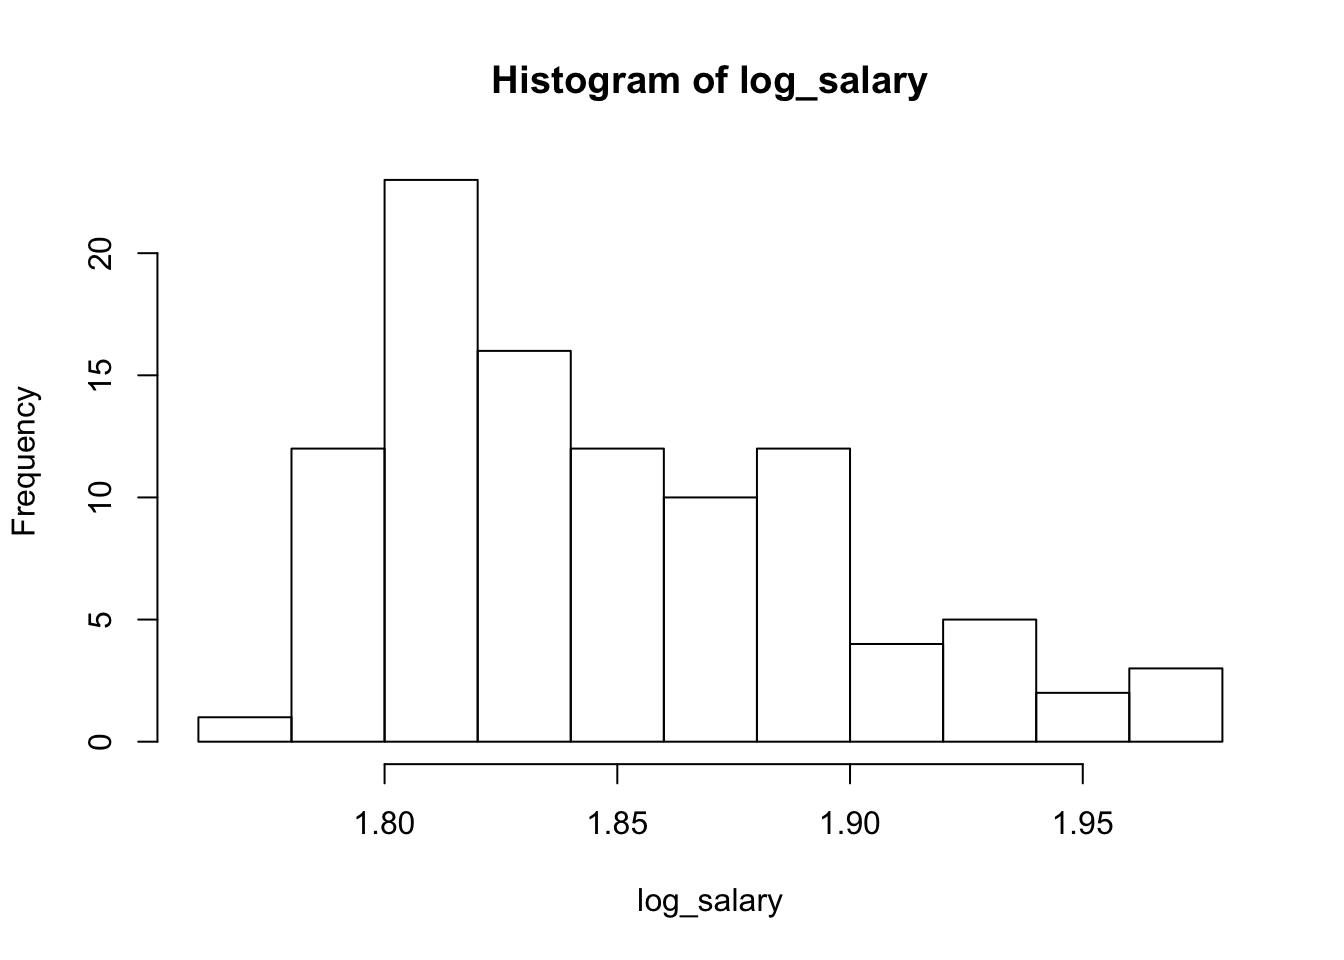
\includegraphics{assignment02-psteinke-timeseries_files/figure-latex/unnamed-chunk-2-1.pdf}

\begin{verbatim}
## 
##  Shapiro-Wilk normality test
## 
## data:  df
## W = 0.94709, p-value = 0.5948
\end{verbatim}

The Box-Cox transformation \textbf{did} help to improve the normality of
the series because: - the dots are more aligned with the red line in the
QQ plot (than solely with the Box-Cox transformation) - the Shapiro test
p-value(0.5948) \textgreater{} 0.05

From ACF and PACF: \texttt{\{arima(p,d,q)\}\ =\ \{arima(1,4,1)\}}

\begin{Shaded}
\begin{Highlighting}[]
\KeywordTok{fig_nums}\NormalTok{(}\StringTok{'Eacf test'}\NormalTok{, }\StringTok{'Eacf test'}\NormalTok{) }\OperatorTok\StringTok{ }\KeywordTok{cat}\NormalTok{()}
\end{Highlighting}
\end{Shaded}

\begin{verbatim}
## Figure  7: Eacf test
\end{verbatim}

\begin{Shaded}
\begin{Highlighting}[]
\KeywordTok{eacf}\NormalTok{(data.ts.boxcox, }\DataTypeTok{ar.max=}\DecValTok{3}\NormalTok{, }\DataTypeTok{ma.max=}\DecValTok{3}\NormalTok{)}
\end{Highlighting}
\end{Shaded}

\begin{verbatim}
## AR/MA
##   0 1 2 3
## 0 x o o o
## 1 o o o o
## 2 o o o o
## 3 o o o o
\end{verbatim}

From the eacf plot we can select: - \texttt{\{arima(0,4,1)\}} -
\texttt{\{arima(1,4,0)\}}

We can also select the following values which are close to the shelf: -
\texttt{\{arima(1,4,1)\}} - \texttt{\{arima(2,4,0)\}}

\hypertarget{residuals-bic-table}{%
\subsection{\texorpdfstring{Residuals: \texttt{BIC}
Table}{Residuals: BIC Table}}\label{residuals-bic-table}}

\begin{Shaded}
\begin{Highlighting}[]
\KeywordTok{fig_nums}\NormalTok{(}\StringTok{'Residual BIC Table'}\NormalTok{, }\StringTok{'Residual BIC table'}\NormalTok{) }\OperatorTok\StringTok{ }\KeywordTok{cat}\NormalTok{()}
\end{Highlighting}
\end{Shaded}

\begin{verbatim}
## Figure  8: Residual BIC table
\end{verbatim}

\begin{Shaded}
\begin{Highlighting}[]
\KeywordTok{par}\NormalTok{(}\DataTypeTok{mfrow=}\KeywordTok{c}\NormalTok{(}\DecValTok{1}\NormalTok{,}\DecValTok{1}\NormalTok{))}
\KeywordTok{armasubsets}\NormalTok{(}\DataTypeTok{y=}\NormalTok{data.ts,}\DataTypeTok{nar=}\DecValTok{3}\NormalTok{,}\DataTypeTok{nma=}\DecValTok{3}\NormalTok{,}\DataTypeTok{y.name=}\StringTok{'test'}\NormalTok{,}\DataTypeTok{ar.method=}\StringTok{'ols'}\NormalTok{) }\OperatorTok\StringTok{ }\KeywordTok{plot}\NormalTok{()}
\end{Highlighting}
\end{Shaded}

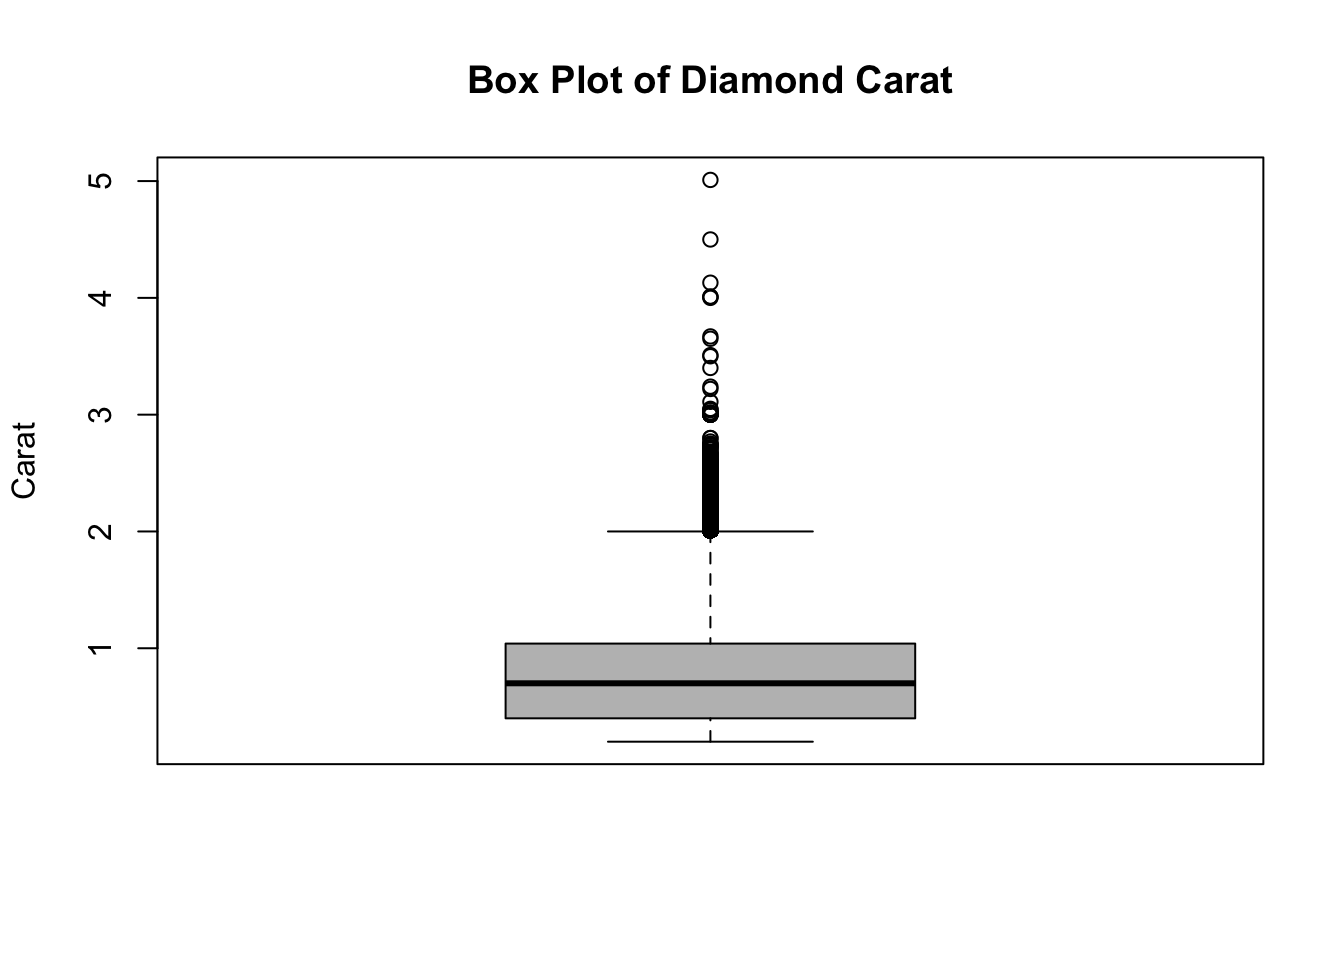
\includegraphics{assignment02-psteinke-timeseries_files/figure-latex/unnamed-chunk-4-1.pdf}

From the \texttt{BIC} residual plot, we can also extract the models:
\texttt{\{arima(1,4,2)\},\ \{arima(1,4,1)\},\ \{arima(0,4,2)\},\ \{arima(0,4,1)\}}
Note: arima(0,4,1) is duplicated in eacf plot

The final set of possible models \texttt{\{arima(p,d,q)\}} is:
\texttt{\{arima(1,4,1),\ arima(0,4,1),\ arima(1,4,0),\ arima(1,4,2)\},\ \{arima(0,4,2)\},\ \{arima(2,4,0)\}}

\hypertarget{arima-model}{%
\subsection{Arima Model}\label{arima-model}}

\begin{Shaded}
\begin{Highlighting}[]
\NormalTok{getModelCoef <-}\StringTok{ }\ControlFlowTok{function}\NormalTok{(pdq) \{}
  \KeywordTok{cat}\NormalTok{(}\StringTok{'}\CharTok{\textbackslash{}n}\StringTok{model: arima('}\NormalTok{, pdq, }\StringTok{')}\CharTok{\textbackslash{}n}\StringTok{'}\NormalTok{)}
\NormalTok{  methods=}\KeywordTok{c}\NormalTok{(}\StringTok{'CSS'}\NormalTok{,}\StringTok{'ML'}\NormalTok{)}
  \ControlFlowTok{for}\NormalTok{ (i }\ControlFlowTok{in}\NormalTok{ methods) \{}
    \KeywordTok{cat}\NormalTok{(i, }\StringTok{'}\CharTok{\textbackslash{}n}\StringTok{'}\NormalTok{)}
\NormalTok{    model =}\StringTok{ }\KeywordTok{arima}\NormalTok{(data.ts,}\DataTypeTok{order=}\NormalTok{pdq,}\DataTypeTok{method=}\NormalTok{i)}
\NormalTok{    coef =}\StringTok{ }\KeywordTok{coeftest}\NormalTok{(model)}
\NormalTok{    modelName <-}\StringTok{ }\KeywordTok{paste}\NormalTok{(}\StringTok{"model"}\NormalTok{, i, }\DataTypeTok{sep =} \StringTok{""}\NormalTok{)}
\NormalTok{    modelToScore <-}\StringTok{ }\KeywordTok{assign}\NormalTok{(modelName, model)}
\NormalTok{    totalResultLines <-}\StringTok{ }\NormalTok{pdq[}\DecValTok{1}\NormalTok{] }\OperatorTok{+}\StringTok{ }\NormalTok{pdq[}\DecValTok{3}\NormalTok{]}
\NormalTok{    startResult <-}\StringTok{ }\NormalTok{totalResultLines}\OperatorTok{*}\DecValTok{3}\CommentTok{# because coeftest() returns a s4 object}
\NormalTok{    pValues <-}\StringTok{ }\DecValTok{1}\OperatorTok{:}\NormalTok{totalResultLines }\OperatorTok
\StringTok{      }\KeywordTok{map}\NormalTok{(}\OperatorTok{~}\StringTok{ }\NormalTok{\{}\KeywordTok{coeftest}\NormalTok{(model)[(.x }\OperatorTok{+}\StringTok{ }\NormalTok{startResult)] }\OperatorTok\StringTok{ }\KeywordTok{round}\NormalTok{(}\DecValTok{6}\NormalTok{) }\OperatorTok\StringTok{ }\KeywordTok{paste}\NormalTok{()\})}
\NormalTok{    isPSignifcant <-}\StringTok{ }\ControlFlowTok{function}\NormalTok{(p) \{ }
      \KeywordTok{ifelse}\NormalTok{(p }\OperatorTok{<}\StringTok{ }\FloatTok{0.05}\NormalTok{, }\StringTok{'p < 0.05 significant'}\NormalTok{, }\StringTok{'p > 0.05 insignificant'}\NormalTok{)}
\NormalTok{    \}}
\NormalTok{    pValues }\OperatorTok\StringTok{ }\KeywordTok{rbind}\NormalTok{(}\KeywordTok{isPSignifcant}\NormalTok{(pValues), }\StringTok{'}\CharTok{\textbackslash{}n}\StringTok{'}\NormalTok{) }\OperatorTok\StringTok{ }\KeywordTok{paste}\NormalTok{() }\OperatorTok\StringTok{ }\KeywordTok{cat}\NormalTok{()}
\NormalTok{  \}}
\NormalTok{\}}
\KeywordTok{cat}\NormalTok{(}\StringTok{'Arima Model coeff p-values (rounded to 6 decimal places):}\CharTok{\textbackslash{}n}\StringTok{'}\NormalTok{)}
\end{Highlighting}
\end{Shaded}

\begin{verbatim}
## Arima Model coeff p-values (rounded to 6 decimal places):
\end{verbatim}

\begin{Shaded}
\begin{Highlighting}[]
\NormalTok{model_}\DecValTok{041}\NormalTok{_p <-}\StringTok{ }\KeywordTok{getModelCoef}\NormalTok{(}\DataTypeTok{pdq=}\KeywordTok{c}\NormalTok{(}\DecValTok{0}\NormalTok{,}\DecValTok{4}\NormalTok{,}\DecValTok{1}\NormalTok{))}
\end{Highlighting}
\end{Shaded}

\begin{verbatim}
## 
## model: arima( 0 4 1 )
## CSS 
## 0 p < 0.05 significant 
## ML 
## 2e-06 p < 0.05 significant
\end{verbatim}

\begin{Shaded}
\begin{Highlighting}[]
\NormalTok{model_}\DecValTok{042}\NormalTok{_p <-}\StringTok{ }\KeywordTok{getModelCoef}\NormalTok{(}\DataTypeTok{pdq=}\KeywordTok{c}\NormalTok{(}\DecValTok{0}\NormalTok{,}\DecValTok{4}\NormalTok{,}\DecValTok{2}\NormalTok{))}
\end{Highlighting}
\end{Shaded}

\begin{verbatim}
## 
## model: arima( 0 4 2 )
## CSS 
## 0 p < 0.05 significant 
##  0 p < 0.05 significant 
## ML 
## 0 p < 0.05 significant 
##  0.003161 p < 0.05 significant
\end{verbatim}

\begin{Shaded}
\begin{Highlighting}[]
\NormalTok{model_}\DecValTok{140}\NormalTok{_p <-}\StringTok{ }\KeywordTok{getModelCoef}\NormalTok{(}\DataTypeTok{pdq=}\KeywordTok{c}\NormalTok{(}\DecValTok{1}\NormalTok{,}\DecValTok{4}\NormalTok{,}\DecValTok{0}\NormalTok{))}
\end{Highlighting}
\end{Shaded}

\begin{verbatim}
## 
## model: arima( 1 4 0 )
## CSS 
## 1e-06 p < 0.05 significant 
## ML 
## 0 p < 0.05 significant
\end{verbatim}

\begin{Shaded}
\begin{Highlighting}[]
\NormalTok{model_}\DecValTok{141}\NormalTok{_p <-}\StringTok{ }\KeywordTok{getModelCoef}\NormalTok{(}\DataTypeTok{pdq=}\KeywordTok{c}\NormalTok{(}\DecValTok{1}\NormalTok{,}\DecValTok{4}\NormalTok{,}\DecValTok{1}\NormalTok{))}
\end{Highlighting}
\end{Shaded}

\begin{verbatim}
## 
## model: arima( 1 4 1 )
## CSS 
## 0.001172 p < 0.05 significant 
##  0 p < 0.05 significant 
## ML 
## 0.001061 p < 0.05 significant 
##  4.3e-05 p < 0.05 significant
\end{verbatim}

\begin{Shaded}
\begin{Highlighting}[]
\NormalTok{model_}\DecValTok{142}\NormalTok{_p <-}\StringTok{ }\KeywordTok{getModelCoef}\NormalTok{(}\DataTypeTok{pdq=}\KeywordTok{c}\NormalTok{(}\DecValTok{1}\NormalTok{,}\DecValTok{4}\NormalTok{,}\DecValTok{2}\NormalTok{))}
\end{Highlighting}
\end{Shaded}

\begin{verbatim}
## 
## model: arima( 1 4 2 )
## CSS 
## 0.147627 p > 0.05 insignificant 
##  0.007886 p < 0.05 significant 
##  0.429623 p > 0.05 insignificant 
## ML 
## 0.239717 p > 0.05 insignificant 
##  5.1e-05 p < 0.05 significant 
##  0.056878 p > 0.05 insignificant
\end{verbatim}

\begin{Shaded}
\begin{Highlighting}[]
\NormalTok{model_}\DecValTok{240}\NormalTok{_p <-}\StringTok{ }\KeywordTok{getModelCoef}\NormalTok{(}\DataTypeTok{pdq=}\KeywordTok{c}\NormalTok{(}\DecValTok{2}\NormalTok{,}\DecValTok{4}\NormalTok{,}\DecValTok{0}\NormalTok{))}
\end{Highlighting}
\end{Shaded}

\begin{verbatim}
## 
## model: arima( 2 4 0 )
## CSS 
## 1e-06 p < 0.05 significant 
##  0.045272 p < 0.05 significant 
## ML 
## 2e-06 p < 0.05 significant 
##  0.053114 p > 0.05 insignificant
\end{verbatim}

\begin{Shaded}
\begin{Highlighting}[]
\NormalTok{model_}\DecValTok{242}\NormalTok{_p <-}\StringTok{ }\KeywordTok{getModelCoef}\NormalTok{(}\DataTypeTok{pdq=}\KeywordTok{c}\NormalTok{(}\DecValTok{2}\NormalTok{,}\DecValTok{4}\NormalTok{,}\DecValTok{1}\NormalTok{))}
\end{Highlighting}
\end{Shaded}

\begin{verbatim}
## 
## model: arima( 2 4 1 )
## CSS 
## 0.000637 p < 0.05 significant 
##  0.215751 p > 0.05 insignificant 
##  5e-06 p < 0.05 significant 
## ML 
## 0.005466 p < 0.05 significant 
##  0.456372 p > 0.05 insignificant 
##  0.00017 p < 0.05 significant
\end{verbatim}

\begin{itemize}
\tightlist
\item
  arima(1,4,2), arima(2,4,1), arima(2,4,0) show insignificant p-values
  \textgreater{} 0.05,
\item
  These are no longer models we will consider
\item
  The remaining models are:
  \texttt{model\_041,\ model\_042,\ model\_140,\ model\_141}
\end{itemize}

\begin{Shaded}
\begin{Highlighting}[]
\NormalTok{model_}\DecValTok{041}\NormalTok{_ml =}\StringTok{ }\KeywordTok{arima}\NormalTok{(data.ts,}\DataTypeTok{order=}\KeywordTok{c}\NormalTok{(}\DecValTok{0}\NormalTok{,}\DecValTok{4}\NormalTok{,}\DecValTok{1}\NormalTok{),}\DataTypeTok{method=}\StringTok{'ML'}\NormalTok{) }\CommentTok{# ARIMA(0,4,1)}
\NormalTok{model_}\DecValTok{042}\NormalTok{_ml =}\StringTok{ }\KeywordTok{arima}\NormalTok{(data.ts,}\DataTypeTok{order=}\KeywordTok{c}\NormalTok{(}\DecValTok{0}\NormalTok{,}\DecValTok{4}\NormalTok{,}\DecValTok{2}\NormalTok{),}\DataTypeTok{method=}\StringTok{'ML'}\NormalTok{) }\CommentTok{# ARIMA(0,4,2)}
\NormalTok{model_}\DecValTok{140}\NormalTok{_ml =}\StringTok{ }\KeywordTok{arima}\NormalTok{(data.ts,}\DataTypeTok{order=}\KeywordTok{c}\NormalTok{(}\DecValTok{1}\NormalTok{,}\DecValTok{4}\NormalTok{,}\DecValTok{0}\NormalTok{),}\DataTypeTok{method=}\StringTok{'ML'}\NormalTok{) }\CommentTok{# ARIMA(1,4,0)}
\NormalTok{model_}\DecValTok{141}\NormalTok{_ml =}\StringTok{ }\KeywordTok{arima}\NormalTok{(data.ts,}\DataTypeTok{order=}\KeywordTok{c}\NormalTok{(}\DecValTok{1}\NormalTok{,}\DecValTok{4}\NormalTok{,}\DecValTok{1}\NormalTok{),}\DataTypeTok{method=}\StringTok{'ML'}\NormalTok{) }\CommentTok{# ARIMA(1,4,1)}

\CommentTok{# AIC and BIC values}
\KeywordTok{sort.score}\NormalTok{(}\KeywordTok{AIC}\NormalTok{(}
\NormalTok{  model_}\DecValTok{041}\NormalTok{_ml, model_}\DecValTok{042}\NormalTok{_ml, model_}\DecValTok{140}\NormalTok{_ml, model_}\DecValTok{141}\NormalTok{_ml ),}
  \DataTypeTok{score =} \StringTok{"aic"}\NormalTok{)}
\end{Highlighting}
\end{Shaded}

\begin{verbatim}
##              df      AIC
## model_042_ml  3 42.84286
## model_141_ml  3 44.37815
## model_140_ml  2 48.87321
## model_041_ml  2 49.07553
\end{verbatim}

\begin{Shaded}
\begin{Highlighting}[]
\KeywordTok{sort.score}\NormalTok{(}\KeywordTok{BIC}\NormalTok{(}
\NormalTok{  model_}\DecValTok{041}\NormalTok{_ml, model_}\DecValTok{042}\NormalTok{_ml, model_}\DecValTok{140}\NormalTok{_ml, model_}\DecValTok{141}\NormalTok{_ml ),}
  \DataTypeTok{score =} \StringTok{"bic"}\NormalTok{)}
\end{Highlighting}
\end{Shaded}

\begin{verbatim}
##              df      BIC
## model_042_ml  3 44.29758
## model_141_ml  3 45.83287
## model_140_ml  2 49.84302
## model_041_ml  2 50.04535
\end{verbatim}

\begin{itemize}
\tightlist
\item
  arimia(0,4,2) ranks highest according to he \texttt{sort.score}
  formula in both AIC and BIC
\end{itemize}

\begin{Shaded}
\begin{Highlighting}[]
\CommentTok{# arima(0,4,2) entire coeficient's output for for completeness:}
\KeywordTok{arima}\NormalTok{(data.ts,}\DataTypeTok{order=}\KeywordTok{c}\NormalTok{(}\DecValTok{0}\NormalTok{,}\DecValTok{4}\NormalTok{,}\DecValTok{2}\NormalTok{),}\DataTypeTok{method=}\StringTok{'ML'}\NormalTok{) }\OperatorTok\StringTok{ }\KeywordTok{coeftest}\NormalTok{()}
\end{Highlighting}
\end{Shaded}

\begin{verbatim}
## 
## z test of coefficients:
## 
##     Estimate Std. Error z value  Pr(>|z|)    
## ma1 -1.86751    0.32411 -5.7619 8.317e-09 ***
## ma2  0.94443    0.31996  2.9517  0.003161 ** 
## ---
## Signif. codes:  0 '***' 0.001 '**' 0.01 '*' 0.05 '.' 0.1 ' ' 1
\end{verbatim}

\hypertarget{residuals}{%
\subsection{Residuals}\label{residuals}}

\begin{Shaded}
\begin{Highlighting}[]
\NormalTok{residual.analysis <-}\StringTok{ }\ControlFlowTok{function}\NormalTok{(model, }\DataTypeTok{std =} \OtherTok{TRUE}\NormalTok{)\{}
  \ControlFlowTok{if}\NormalTok{ (std }\OperatorTok{==}\StringTok{ }\OtherTok{TRUE}\NormalTok{)\{}
\NormalTok{    res.model =}\StringTok{ }\KeywordTok{rstandard}\NormalTok{(model)}
\NormalTok{  \}}\ControlFlowTok{else}\NormalTok{\{}
\NormalTok{    res.model =}\StringTok{ }\KeywordTok{residuals}\NormalTok{(model)}
\NormalTok{  \}}
  \KeywordTok{par}\NormalTok{(}\DataTypeTok{mfrow=}\KeywordTok{c}\NormalTok{(}\DecValTok{3}\NormalTok{,}\DecValTok{2}\NormalTok{),}
      \DataTypeTok{oma =} \KeywordTok{c}\NormalTok{(}\DecValTok{1}\NormalTok{,}\DecValTok{1}\NormalTok{,}\DecValTok{0}\NormalTok{,}\DecValTok{0}\NormalTok{) }\OperatorTok{+}\StringTok{ }\FloatTok{0.1}\NormalTok{,}
      \DataTypeTok{mar =} \KeywordTok{c}\NormalTok{(}\DecValTok{2}\NormalTok{,}\DecValTok{2}\NormalTok{,}\DecValTok{2}\NormalTok{,}\DecValTok{2}\NormalTok{) }\OperatorTok{+}\StringTok{ }\FloatTok{0.1}\NormalTok{)}
  \KeywordTok{plot}\NormalTok{(}
\NormalTok{    res.model,}
    \DataTypeTok{type=}\StringTok{'o'}\NormalTok{,}
    \DataTypeTok{xlab=}\StringTok{'years'}\NormalTok{,}
    \DataTypeTok{ylab=}\StringTok{'Standardised residuals'}\NormalTok{,}
    \DataTypeTok{main=}\StringTok{"Time series plot of standardised residuals"}\NormalTok{)}
  \KeywordTok{abline}\NormalTok{(}\DataTypeTok{h=}\DecValTok{0}\NormalTok{)}
  \KeywordTok{hist}\NormalTok{(res.model,}\DataTypeTok{main=}\StringTok{"Histogram of standardised residuals"}\NormalTok{)}
  \KeywordTok{qqnorm}\NormalTok{(res.model,}\DataTypeTok{main=}\StringTok{"QQ plot of standardised residuals"}\NormalTok{)}
  \KeywordTok{qqline}\NormalTok{(res.model, }\DataTypeTok{col =} \DecValTok{2}\NormalTok{)}
  \KeywordTok{acf}\NormalTok{(res.model,}\DataTypeTok{main=}\StringTok{"ACF of standardised residuals"}\NormalTok{)}
  \KeywordTok{print}\NormalTok{(}\KeywordTok{shapiro.test}\NormalTok{(res.model))}
\NormalTok{  k=}\DecValTok{0}
  \KeywordTok{LBQPlot}\NormalTok{(res.model, }\DataTypeTok{lag.max =} \KeywordTok{length}\NormalTok{(model}\OperatorTok{$}\NormalTok{residuals)}\OperatorTok{-}\DecValTok{1}\NormalTok{ , }\DataTypeTok{StartLag =}\NormalTok{ k }\OperatorTok{+}\StringTok{ }\DecValTok{1}\NormalTok{, }\DataTypeTok{k =} \DecValTok{0}\NormalTok{, }\DataTypeTok{SquaredQ =} \OtherTok{FALSE}\NormalTok{)}
  \CommentTok{#resPlotsTitle <- paste('Figure', figureCount, '. Standardised residuals of ', default_ylab, sep = '')}
  \CommentTok{#title(resPlotsTitle, side = 3, line = -33, outer = TRUE, cex.adj = 3)}
  \CommentTok{#figureCount <- figureCount + 1}
  \KeywordTok{par}\NormalTok{(}\DataTypeTok{mfrow=}\KeywordTok{c}\NormalTok{(}\DecValTok{1}\NormalTok{,}\DecValTok{1}\NormalTok{))}
\NormalTok{\}}
\KeywordTok{fig_nums}\NormalTok{(}\StringTok{'Residual Analysis'}\NormalTok{, }\StringTok{'Residual Analysis'}\NormalTok{) }\OperatorTok\StringTok{ }\KeywordTok{cat}\NormalTok{()}
\end{Highlighting}
\end{Shaded}

\begin{verbatim}
## Figure  9: Residual Analysis
\end{verbatim}

\begin{Shaded}
\begin{Highlighting}[]
\KeywordTok{residual.analysis}\NormalTok{(}\DataTypeTok{model =}\NormalTok{ model_}\DecValTok{042}\NormalTok{_ml)}
\end{Highlighting}
\end{Shaded}

\begin{verbatim}
## 
##  Shapiro-Wilk normality test
## 
## data:  res.model
## W = 0.91548, p-value = 0.1426
\end{verbatim}

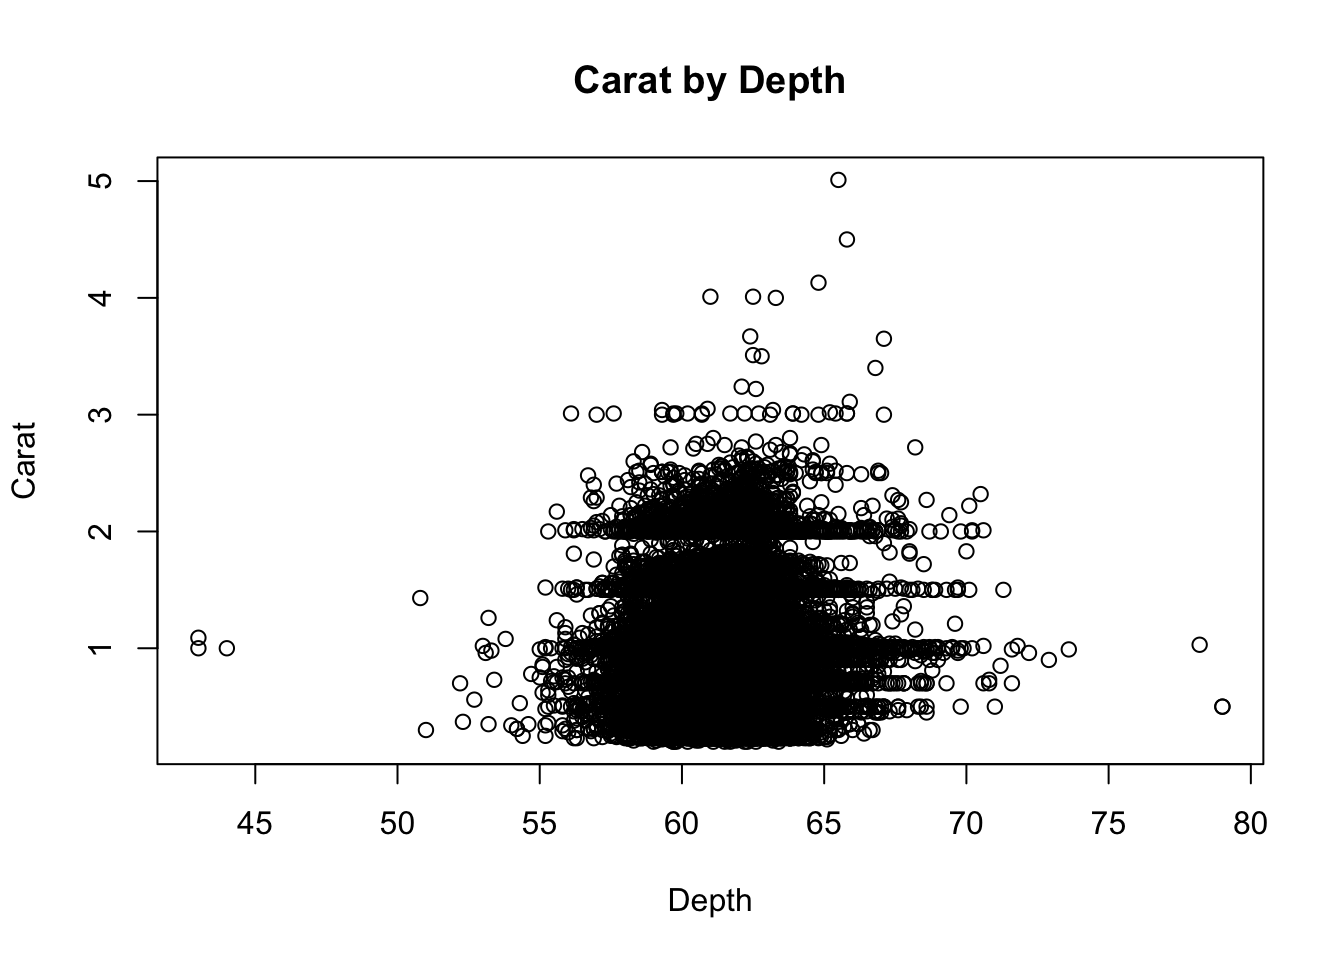
\includegraphics{assignment02-psteinke-timeseries_files/figure-latex/unnamed-chunk-8-1.pdf}

\begin{itemize}
\tightlist
\item
  Time-series standardised residuals: cannot observe a trend
\item
  histogram: data is not normal and left skewed
\item
  Ljung-Box test: all dots \textgreater{} red line
\item
  Q-Q plot: left-tailed, doesn't fit
\item
  ACF: no lags, indicating white noise
\end{itemize}

∴ We cannot make any meaningful timeseries observations from the
residuals, indicating a good model fit

\hypertarget{forecast}{%
\subsection{Forecast}\label{forecast}}

\begin{Shaded}
\begin{Highlighting}[]
\KeywordTok{library}\NormalTok{(forecast)}
\end{Highlighting}
\end{Shaded}

\begin{verbatim}
## Warning: package 'forecast' was built under R version 3.5.2
\end{verbatim}

\begin{Shaded}
\begin{Highlighting}[]
\NormalTok{figureName <-}\StringTok{ }\KeywordTok{fig_nums}\NormalTok{(}\StringTok{'Forecast of growth'}\NormalTok{, }\StringTok{'Forecast of growth'}\NormalTok{) }\OperatorTok\StringTok{ }\KeywordTok{cat}\NormalTok{()}
\end{Highlighting}
\end{Shaded}

\begin{verbatim}
## Figure  10: Forecast of growth
\end{verbatim}

\begin{Shaded}
\begin{Highlighting}[]
\CommentTok{# lambda of 0.35 is from Box-Cox transformation:}
\NormalTok{fit =}\StringTok{ }\KeywordTok{Arima}\NormalTok{(data.ts.raw,}\KeywordTok{c}\NormalTok{(}\DecValTok{0}\NormalTok{,}\DecValTok{4}\NormalTok{,}\DecValTok{2}\NormalTok{), }\DataTypeTok{lambda =}\NormalTok{ lambda) }
\CommentTok{# hack to hide negative values:}
\NormalTok{ylim <-}\StringTok{ }\KeywordTok{c}\NormalTok{(}\DecValTok{500}\NormalTok{, }\DecValTok{14000}\NormalTok{) }
\KeywordTok{plot}\NormalTok{(}
  \KeywordTok{forecast}\NormalTok{(fit,}\DataTypeTok{h=}\DecValTok{10}\NormalTok{), }
   \DataTypeTok{ylim=}\NormalTok{ylim, }
   \DataTypeTok{ylab=}\NormalTok{figureName}
\NormalTok{   )}
\end{Highlighting}
\end{Shaded}

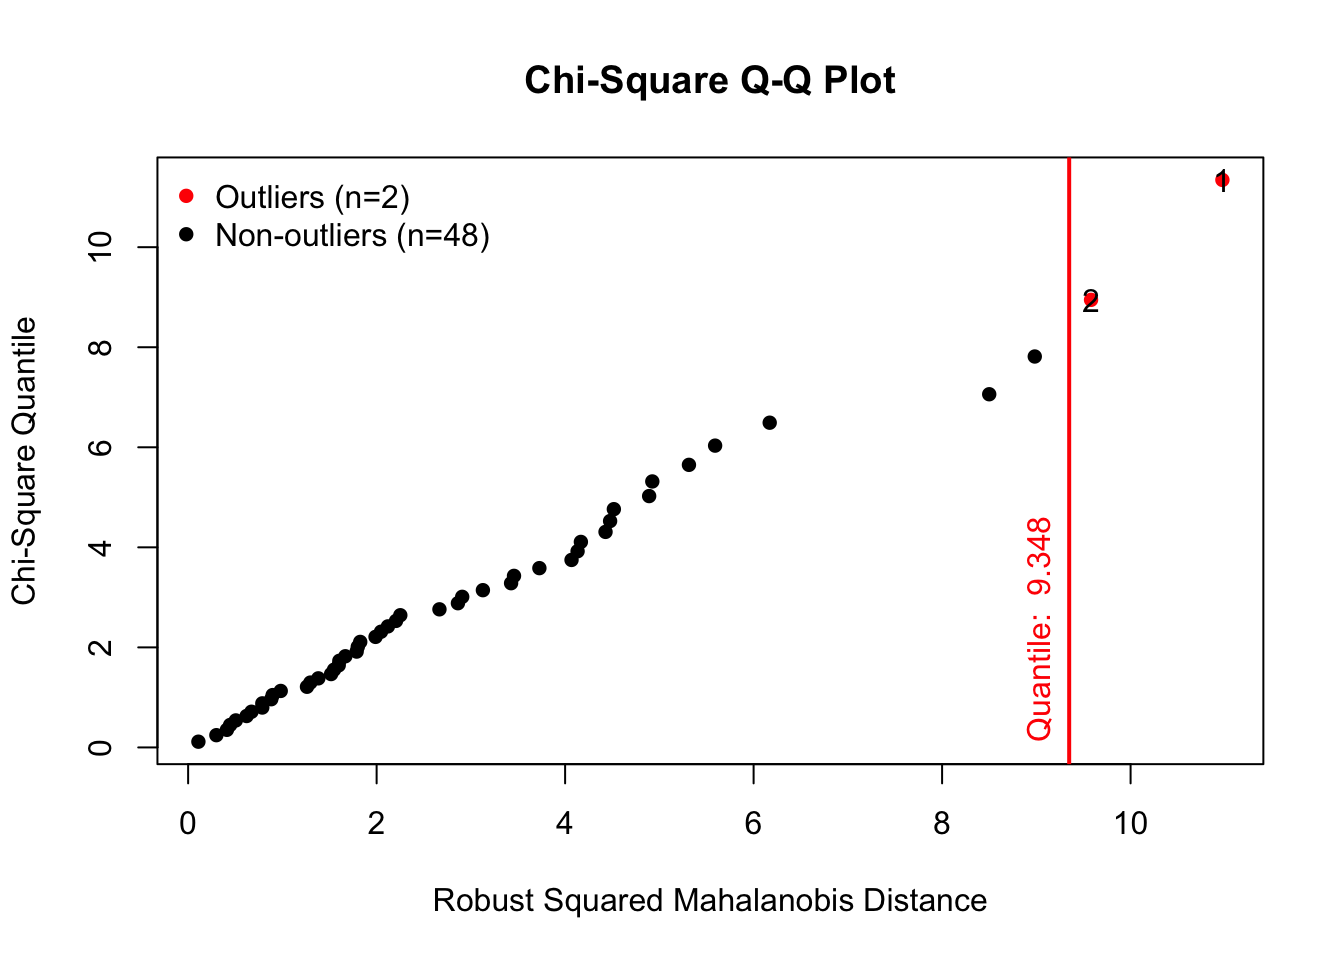
\includegraphics{assignment02-psteinke-timeseries_files/figure-latex/unnamed-chunk-9-1.pdf}

\begin{itemize}
\tightlist
\item
  The forecast shows an almost exponential positive trend in growth,
  with quite a wide confidence interval
\end{itemize}

NOTE: negative trend has been hidden on this plot, because it's not
possible for fish to lay a negative number of eggs. This is a plot
side-effect generated because λ ≠ 0

\hypertarget{conclusion}{%
\subsection{Conclusion}\label{conclusion}}

We have selected \texttt{\{arima(0,4,2)\}} as our best fitting
time-series model

The results of the above tests summarised: -
\texttt{p-value(0.02)\ \textless{}\ 0.05} in our adfTest -
\texttt{ma2\ and\ ma1\ p\ \textless{}\ 0.05} in coefficient test

Please note that the dataset is quite small, so we have limited most of
our decisions to programatic output

The forcast shows a possible 3,000,000,000 eggs laid in 2006. Given the
dataset is limited to 16 values, a more detailed dataset should be
examined to check accuracy of fit. The model may also be adjusted
because of the
\href{https://en.wikipedia.org/wiki/Coregonus_hoyi}{scarcity of food and
high mortality rate of larval Bloaters}

If the model still fits, recommendations include investing in the cavier
industry in Lake Huron


\end{document}
